\documentclass[11pt]{article}
\usepackage{amssymb}
\usepackage{amsmath}
\usepackage{mathrsfs}
\usepackage{bbm}
\usepackage{tikz}
\usepackage{accents}
\usepackage[utf8]{inputenc}
\usepackage[english]{babel}
\usepackage{graphicx}
\usepackage{centernot}
\newcommand{\bs}{{\bigskip}}
\newcommand{\floor}[1]{\lfloor #1 \rfloor}
\newcommand{\ceiling}[1]{\lceil #1 \rceil}
\newcommand{\ms}{{\medskip}}
\newcommand{\sms}{{\smallskip}}
\newcommand{\N}{\mathbb{N}}
\renewcommand{\baselinestretch}{1.5}
\newcommand{\indi}{\mathbbm{1}}
\newcommand{\R}{\mathbb{R}}
\newcommand{\sigF}{\mathcal{F}}
\newcommand{\Z}{\mathbb{Z}}
\newcommand{\C}{\mathbb{C}}
\newcommand{\Q}{\mathbb{Q}}
\newcommand{\E}{\mathbb{E}}
\newcommand{\B}{\mathbb{B}}
\newcommand{\dd}[2]{\frac{d{#1}}{d{#2}}}
\newcommand{\fancyF}{\mathscr{F}}
\newcommand{\borelB}{\mathcal{B}}
\newcommand{\Var}{\text{Var}}
\newcommand{\inner}[2]{\langle{#1},{#2}\rangle}
\newcommand{\sinner}[1]{\langle{#1},{#1} \rangle}
\renewcommand{\epsilon}{\varepsilon}
\renewcommand{\overrightarrow}{\vec}
\newcommand{\tb}{\textbf}
\newcommand{\bfrac}[2]{\displaystyle{\frac{#1}{#2}}}
\newcommand{\bcup}{\bigcup\limits}
\newcommand{\bcap}{\bigcap\limits}
\newcommand{\ceil}[1]{\left\lceil #1 \right\rceil}
\newcommand{\nimply}{\centernot\Rightarrow}
\newcommand{\ar}{\Rightarrow}
\newcommand{\norm}[2]{\| #1 \|_{#2}}
\newcommand{\bnorm}[1]{\norm{#1}{}}
\newcommand{\probp}{\mathbb{P}}
\newcommand{\enorm}[1]{\| #1 \|}
\newcommand{\goto}{\rightarrow}
\newcommand{\bint}[2]{\displaystyle{\int_{#1}^{#2}}}
\newcommand{\nogoto}{\centernot\rightarrow}
\renewcommand{\baselinestretch}{1.5}
\newcommand{\bsum}[2]{\displaystyle{\sum_{#1}^{#2}}}
\newcommand{\bprod}[2]{\displaystyle{\prod_{#1}^{#2}}}
\newcommand{\func}[3]{#1: #2\rightarrow#3}
\newcommand{\sfunc}[2]{#1: #2\rightarrow#2}
\newcommand{\cexp}[2]{\E[#1 \mid #2]}
\usepackage{venndiagram}
\newcommand{\Lim}[1]{\raisebox{0.5ex}{\scalebox{0.8}{$\displaystyle \lim_{#1}\;$}}}
\newcommand{\Limn}{\Lim{n \in \N}}
\newcommand{\Cross}{\mathbin{\tikz [x=1.4ex,y=1.4ex,line width=.2ex] \draw (0,0) -- (1,1) (0,1) -- (1,0);}}
\title{ BA-Sindy}
\author{}
\setlength{\parindent}{0pt}

\begin{document}

\centerline{\tb{Basic description of BA-Sindy algorithm}}

\ms

Inputs:  $X,\dot{X} \in \R^{m \times D}$,   with $\Theta = [\theta_1,...\theta_p]$,  
and $\func{\theta_i}{\R^d}{\R}$

Paramaters:  Pretrain epochs $n_{pre}$,  outer loops epochs $n_{train}$,  inner loop 'bagging' epochs $n_{bag}$,   inner loop train epochs $n_{sub}$, refinement epochs $n_{ref}$

Learning rates for pre-training,  bagging and subtraining, $lr_{pre},  lr_{bag}, lr_{sub}$

Bag size $q$ and  bag number $p$ Loss weightings $\lambda_0 , \lambda_1,  \lambda_2,  \lambda_3$

Activation and bagging thresholds $\epsilon_{act}$ and $\epsilon_{bagg}$.  Noise paramater $\alpha$

\sms

1.  Train regular Sindy autoencoder without sequential thresholding for $n_{pre}$ epochs, learning rate $lr_{pre}$.  This yields an encoder $\func{\zeta_0}{\R^D}{\R^d}$,  a decoder 

$\func{\psi_0}{\R^D}{\R^d}$ and a  Sindy coefficient matrix $\Xi_0 \in \R^{d\times p}$.

Set $\mathcal{L}_{bag} = \lambda_1\mathcal{L}_{dx/dt} +  \lambda_2\mathcal{L}_{dz/dt} + \lambda_3\mathcal{L}_{reg}$

Set $\mathcal{L}_{full} =\lambda_0\mathcal{L}_{encoder} + \lambda_1\mathcal{L}_{dx/dt} +  \lambda_2\mathcal{L}_{dz/dt} + \lambda_3\mathcal{L}_{reg}$

Set coefficient mask $\Lambda^{(0)} = 1^{d\times p}$


2.   Let $i_1,...i_p \subset \{1,...m\}$ and $|i_k| = q$.   Choosen with replacement.   

We typically choose $q = \text{int}(1.5m/p)$
Use indexes $i_1,...i_p$ to create data bags

 $X_{i_1},...X_{i_p}$,  and  
$\dot{X}_{i_1},...\dot{X}_{i_p}$,where $X_{i_k},\dot{X}_{i_k} \in \R^{q \times D}$.  


3.  For $k = 0,... n_{train}$:
 
\hspace{15 pt} For $j = 1,...p$:

\hspace{30 pt} Get $\Xi_{rand} \in \R^{p \times d}$  with $(\Xi_{rand})_{i,j} \sim \mathcal{N}(0,1)$

\hspace{30 pt} $\Xi^{(k,j)}= \text{copy}(\Xi^{(k)})  + \alpha \Xi_{rand}$

\hspace{30 pt}  Update $\Xi^{(k,j)}$ using $\nabla_{\Xi} \mathcal{L}_{bag}(X_{i_j}  \dot{X}_{i_j})$ for $n_{bag}$ epochs,  with $lr_{bag}$


\hspace{15 pt} Set $\Xi^{(k)} = \frac{1}{p} \sum_{j}\Xi^{(k,j)}$ and 
$ \overline{\Lambda}^{(k)} _{i,j} =\indi\{\sum_h\indi \{|\Xi^{(k,h)}_{i,j}|  > \epsilon_{act}\} > \epsilon_{bag} \}$.  


\hspace{15 pt} Set $\Lambda^{(k+1)}  =  \overline{\Lambda}^{(k)} \odot\Lambda^{(k)}$


\hspace{15 pt} Update $\Xi^{(k)},  \zeta^{(k)},  \psi^{(k)},$ using 
$\nabla_{\Xi, \zeta, \psi}\mathcal{L}_{full}(X,\dot{X})$,  for $n_{sub}$ epochs w $lr_{sub}$.


\hspace{15 pt}  Set $\Xi^{(k+1)}, \zeta^{(k+1)}, \psi^{(k+1)} = \Xi^{(k)}, \zeta^{(k)}, \psi^{(k)}$

4.  Update $\Xi^{(n)},  \zeta^{(n)},  \psi^{(n)},$ using 
$\nabla_{\Xi, \zeta, \psi}\mathcal{L}_{full}(X,\dot{X})$,  for $n_{ref}$ epochs w $lr_{sub}$.


\pagebreak

\centerline{\tb{Preliminary results on Lorentz system}}

Train \& test data was of dim $128 \times 5000$, generated from Lorentz system.
 Loss and coefficient count for each averaged over 5 runs is given below.


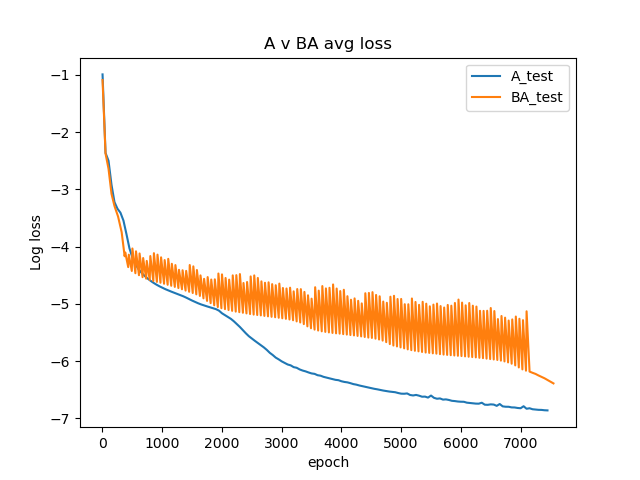
\includegraphics[width=100mm]{avg_loss.png}



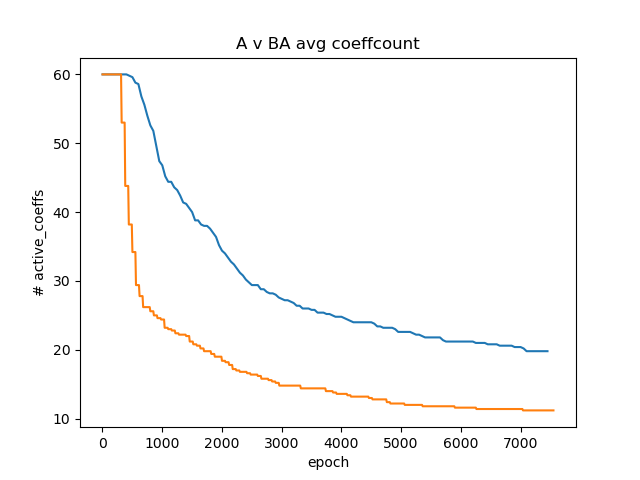
\includegraphics[width=100mm]{avg_coeff.png}


\pagebreak

On some runs we uniformly beat regular auto encoder Sindy,  achieving 

better test loss greater sparsity for the same \# of epochs. Examples below:


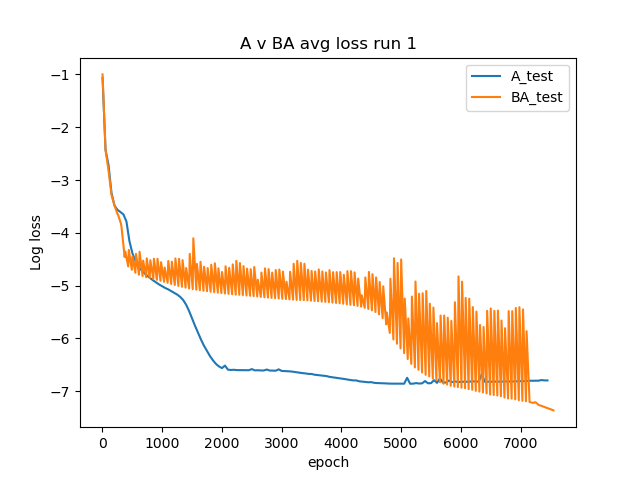
\includegraphics[width=80mm]{run1_loss.png}
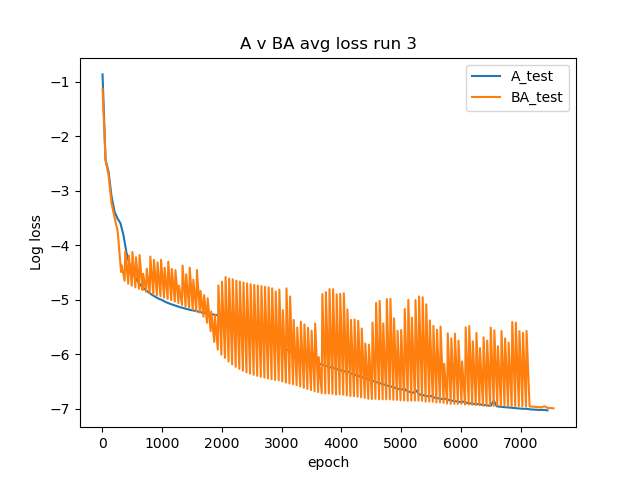
\includegraphics[width=80mm]{run3_loss.png}

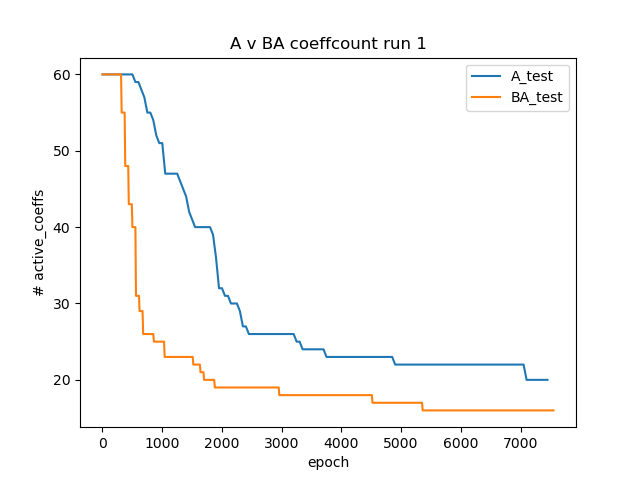
\includegraphics[width=80mm]{run1_coeffs.png}
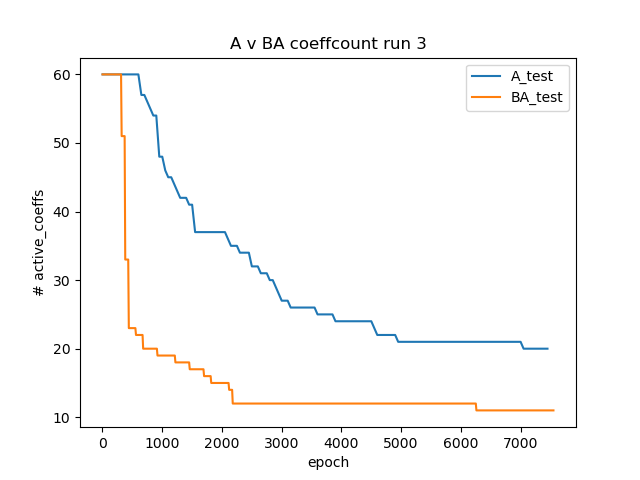
\includegraphics[width=80mm]{run3_coeffs.png}




   

\end{document}